\documentclass{standalone}
\usepackage{tikz}
\usepackage{xcolor}

% Define colors
\definecolor{blueStudent}{RGB}{0, 0, 255} % Blue for female students
\definecolor{redStudent}{RGB}{255, 0, 0}   % Red for male students

\begin{document}

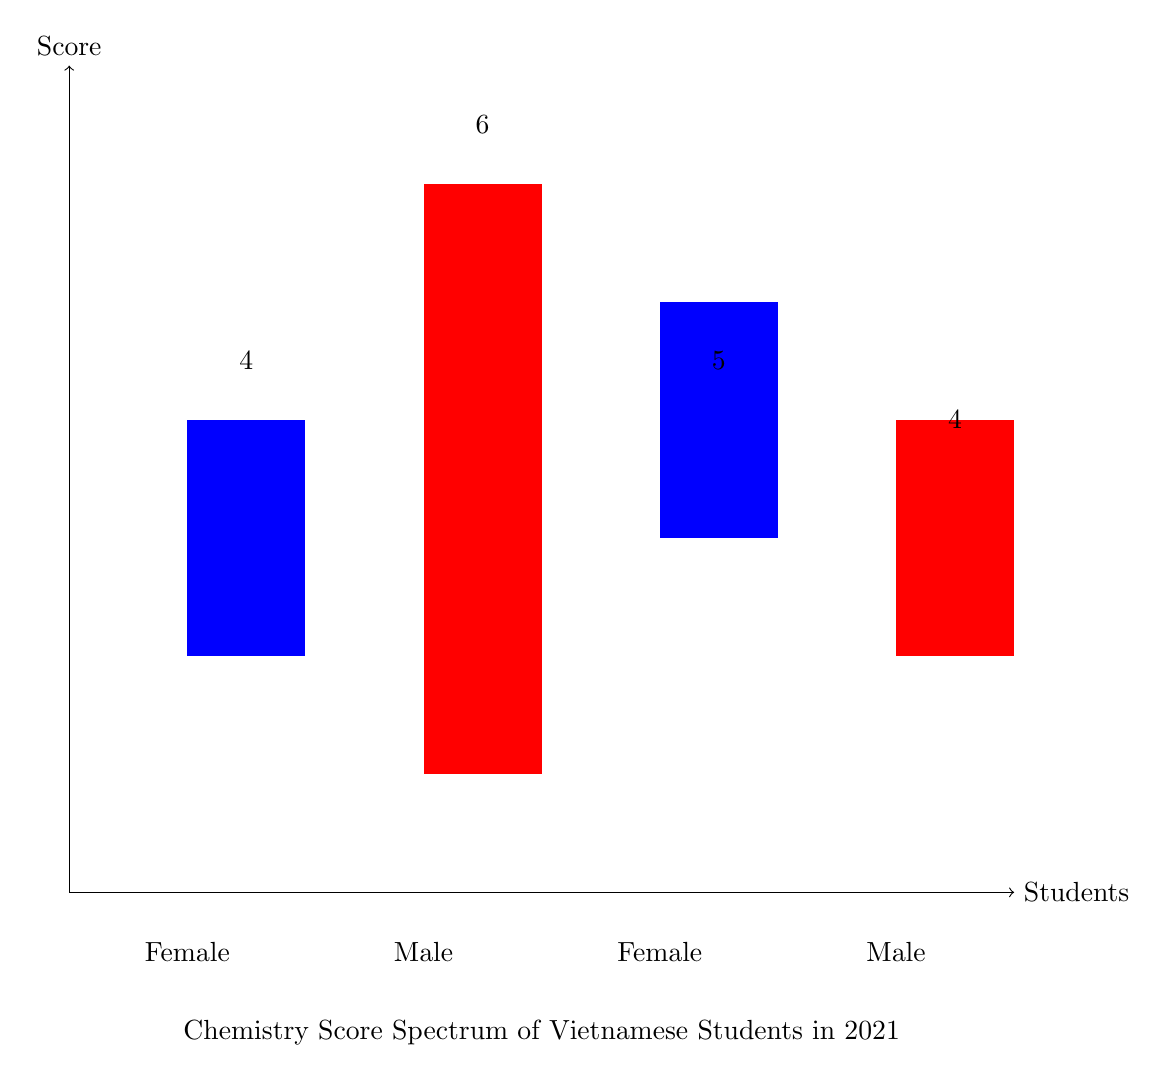
\begin{tikzpicture}[scale=1.5]
    % Draw x-axis
    \draw[->] (0,0) -- (8,0) node[right] {Students};
    
    % Draw y-axis
    \draw[->] (0,0) -- (0,7) node[above] {Score};
    
    % Draw labels
    \foreach \x/\y in {1/Female, 3/Male, 5/Female, 7/Male}{
        \node at (\x,-0.5) {\y};
    }
    
    % Draw bars
    \fill[blueStudent] (1,2) rectangle (2,4);
    \fill[redStudent] (3,1) rectangle (4,6);
    \fill[blueStudent] (5,3) rectangle (6,5);
    \fill[redStudent] (7,2) rectangle (8,4);
    
    % Draw value labels
    \node at (1.5,4.5) {4};
    \node at (3.5,6.5) {6};
    \node at (5.5,4.5) {5};
    \node at (7.5,4) {4};
    
    % Title
    \node at (4,-1) [below] {Chemistry Score Spectrum of Vietnamese Students in 2021};
\end{tikzpicture}

\end{document}